Programe en su lenguaje favorito.
Necesitará (al menos) funciones que hagan lo siguiente:
\begin{itemize}
	\item Generar una secuencia aleatoria de 200 bases
		equiprobables e independientes.
		Nos interesa la evolución de una especie alienígena
		en que las bases del DNA son 6, no 4: $A,C,G,T,B,D$.

	\item Una función que aplique una mutación a una secuencia;
		la mutación se escoge entre inserción, borrado y reemplazo
		de manera equiprobable, y su lugar de aplicación se elige
		al azar a lo largo de la secuencia.

		\begin{itemize}
			\item El borrado borra una letra,
			\item la inserción inserta una letra (equiprobable),
			\item el reemplazo reemplaza una letra por cualquiera
				de las otras 5 (de manera equiprobable).
		\end{itemize}

	\item Una función que calcule la distancia de Levenshtein
		entre dos secuencias (implementando Needleman-Wunsch).
\end{itemize}

Con esas funciones, hará lo siguiente:

\red{Importante:} Las funciones se encuentran en el Anexo 1~\ref{sec:anexo1}.

\begin{enumerate}

	\item Generar una secuencia, y aplicar M mutaciones; para M entre 0 y 300, grafique la relación
		entre M y D, donde D es la distancia de Levenshtein entre la secuencia final y la secuencia
		inicial.

		\blue{Respuesta:}

		\begin{center}
			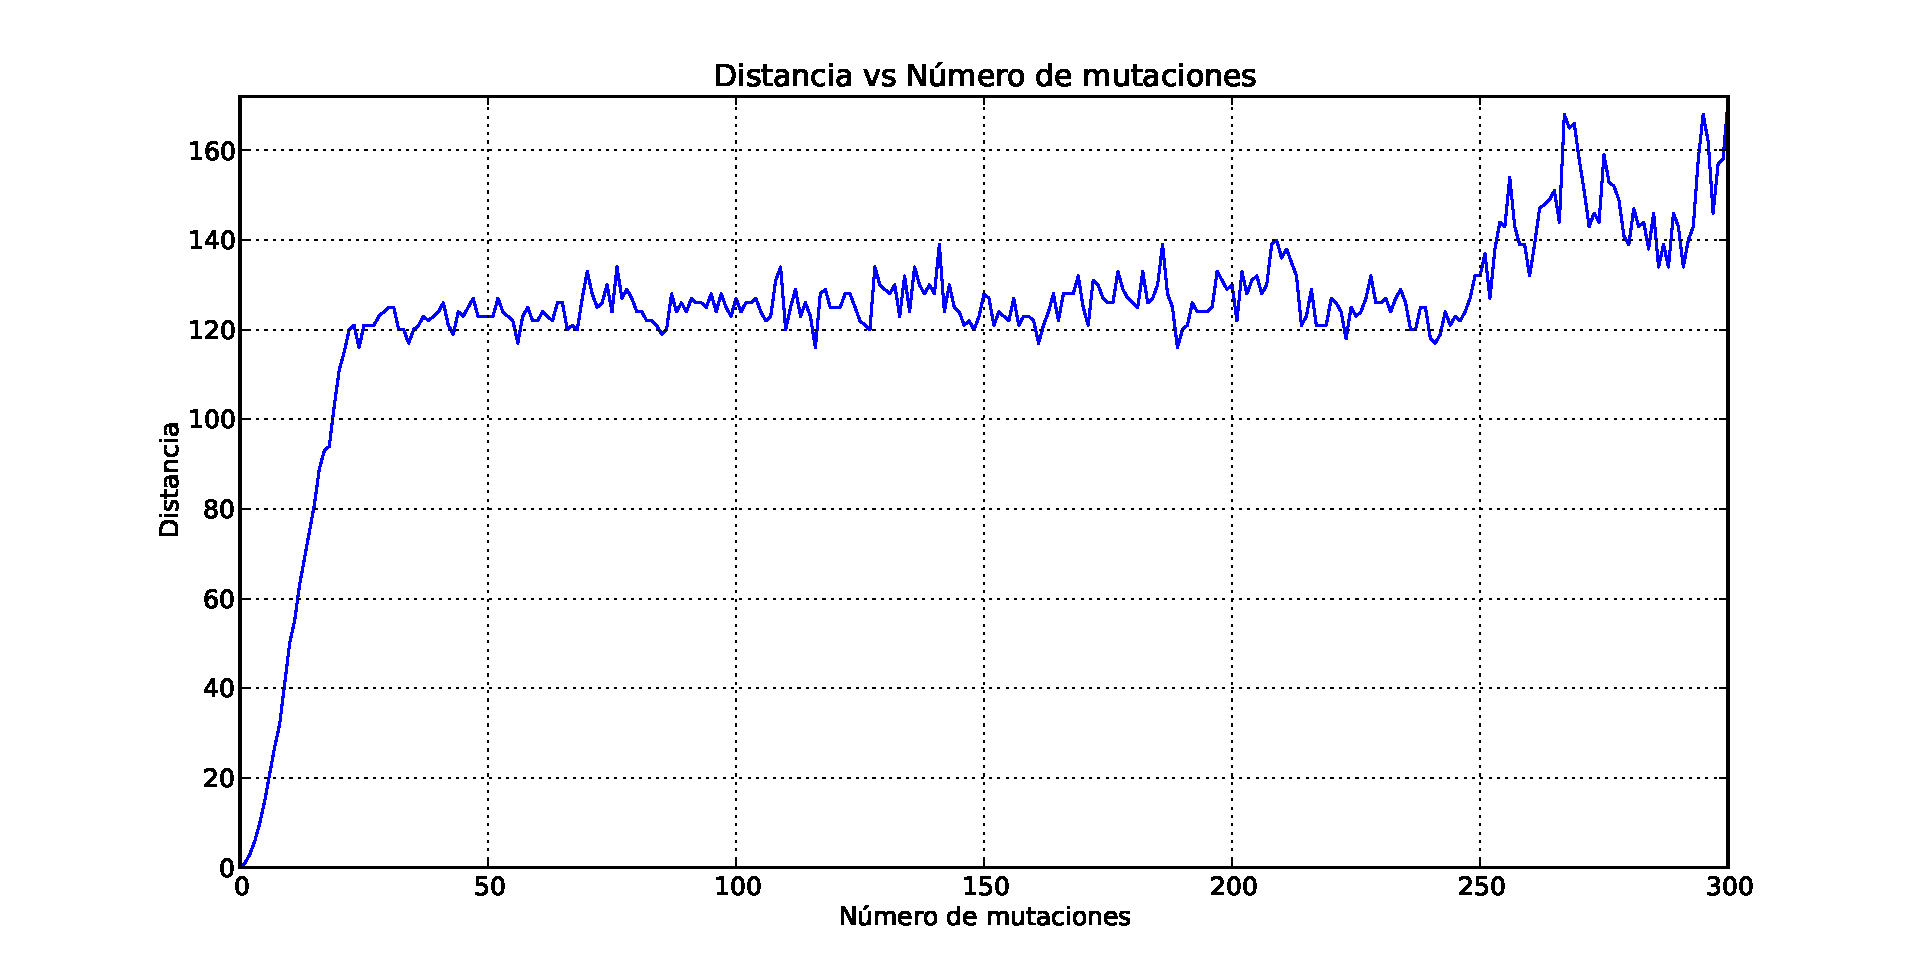
\includegraphics[width=\textwidth]{scripts/pregunta-2-1.pdf}
		\end{center}


	\item Genere una secuencia, clónela, y a cada copia aplíquele M mutaciones (de modo que tendrá
		dos secuencias crecientemente distintas). Grafique la relación entre M y D’, donde D’ es la
		distancia entre las dos secuencias que están mutando.

		\blue{Respuesta:}

		\begin{center}
			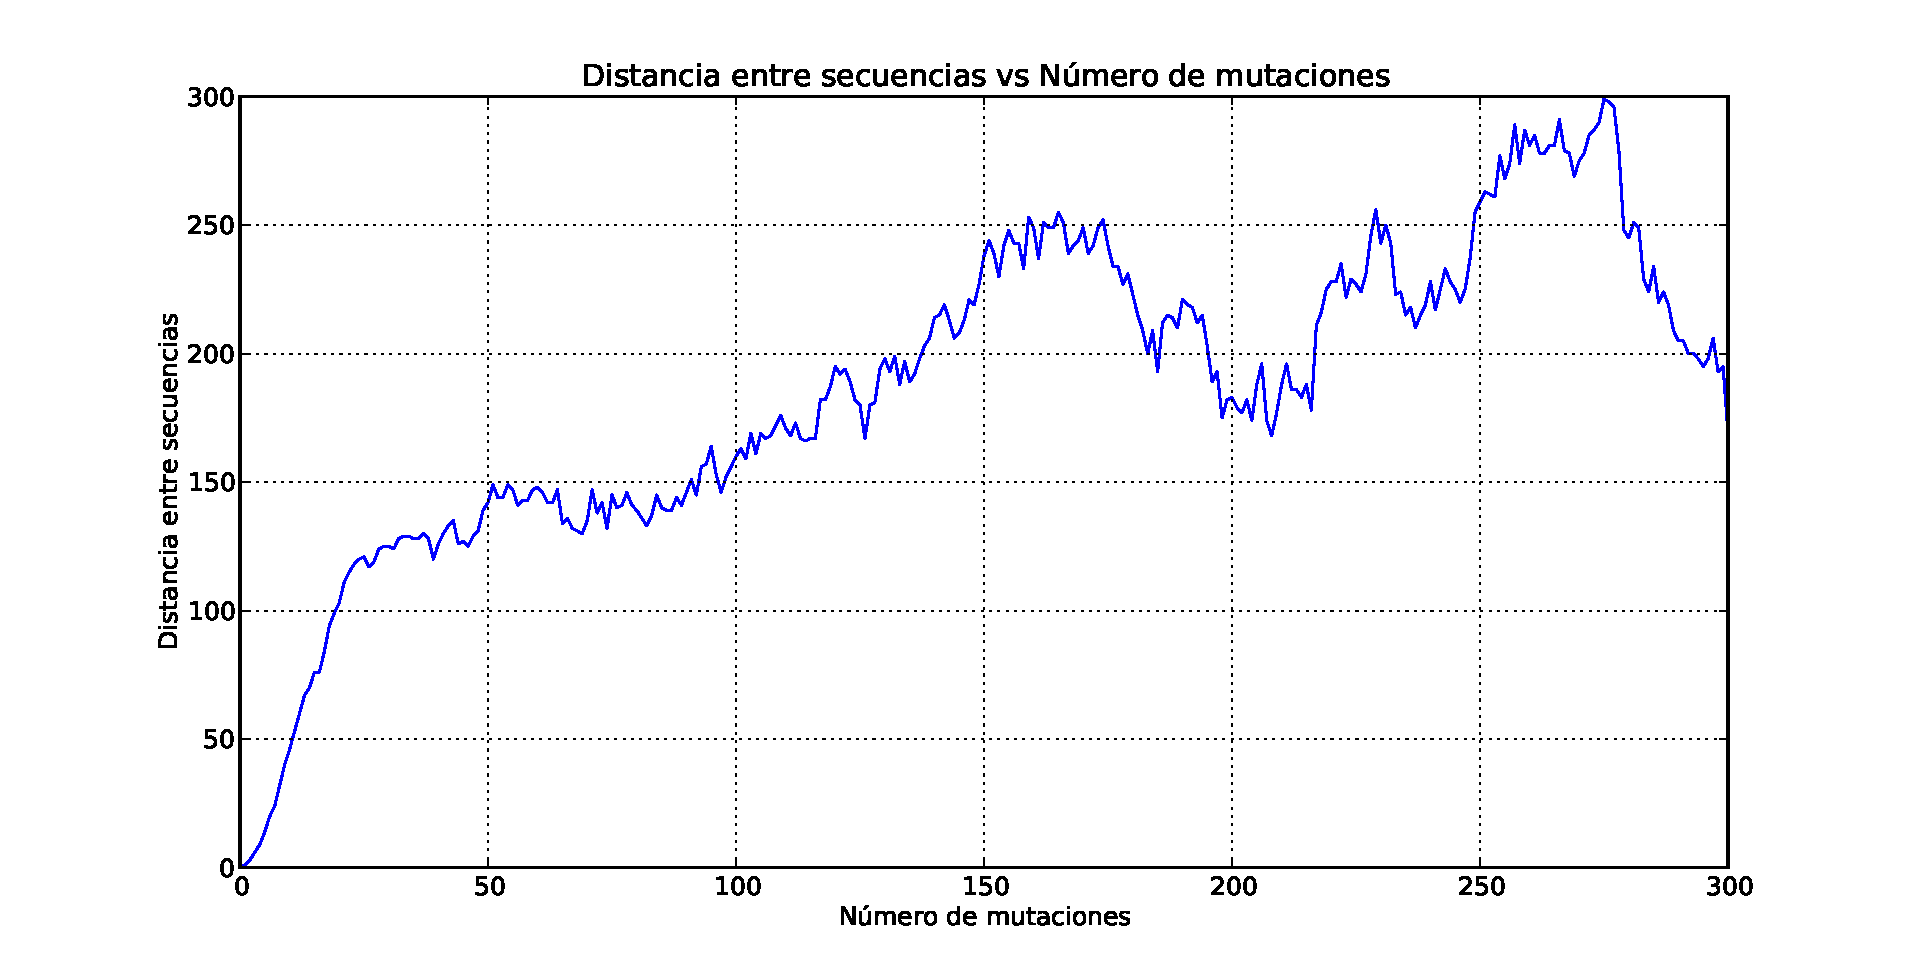
\includegraphics[width=\textwidth]{scripts/pregunta-2-2.pdf}
		\end{center}


	\item Genere 10.000 pares de secuencias (largo 200 c/u) y evalúe su distancia de Levenshtein; haga
		un histograma de la distribución de estos valores, y calcule media y $\sigma$

		\blue{Respuesta:}

		\begin{center}
			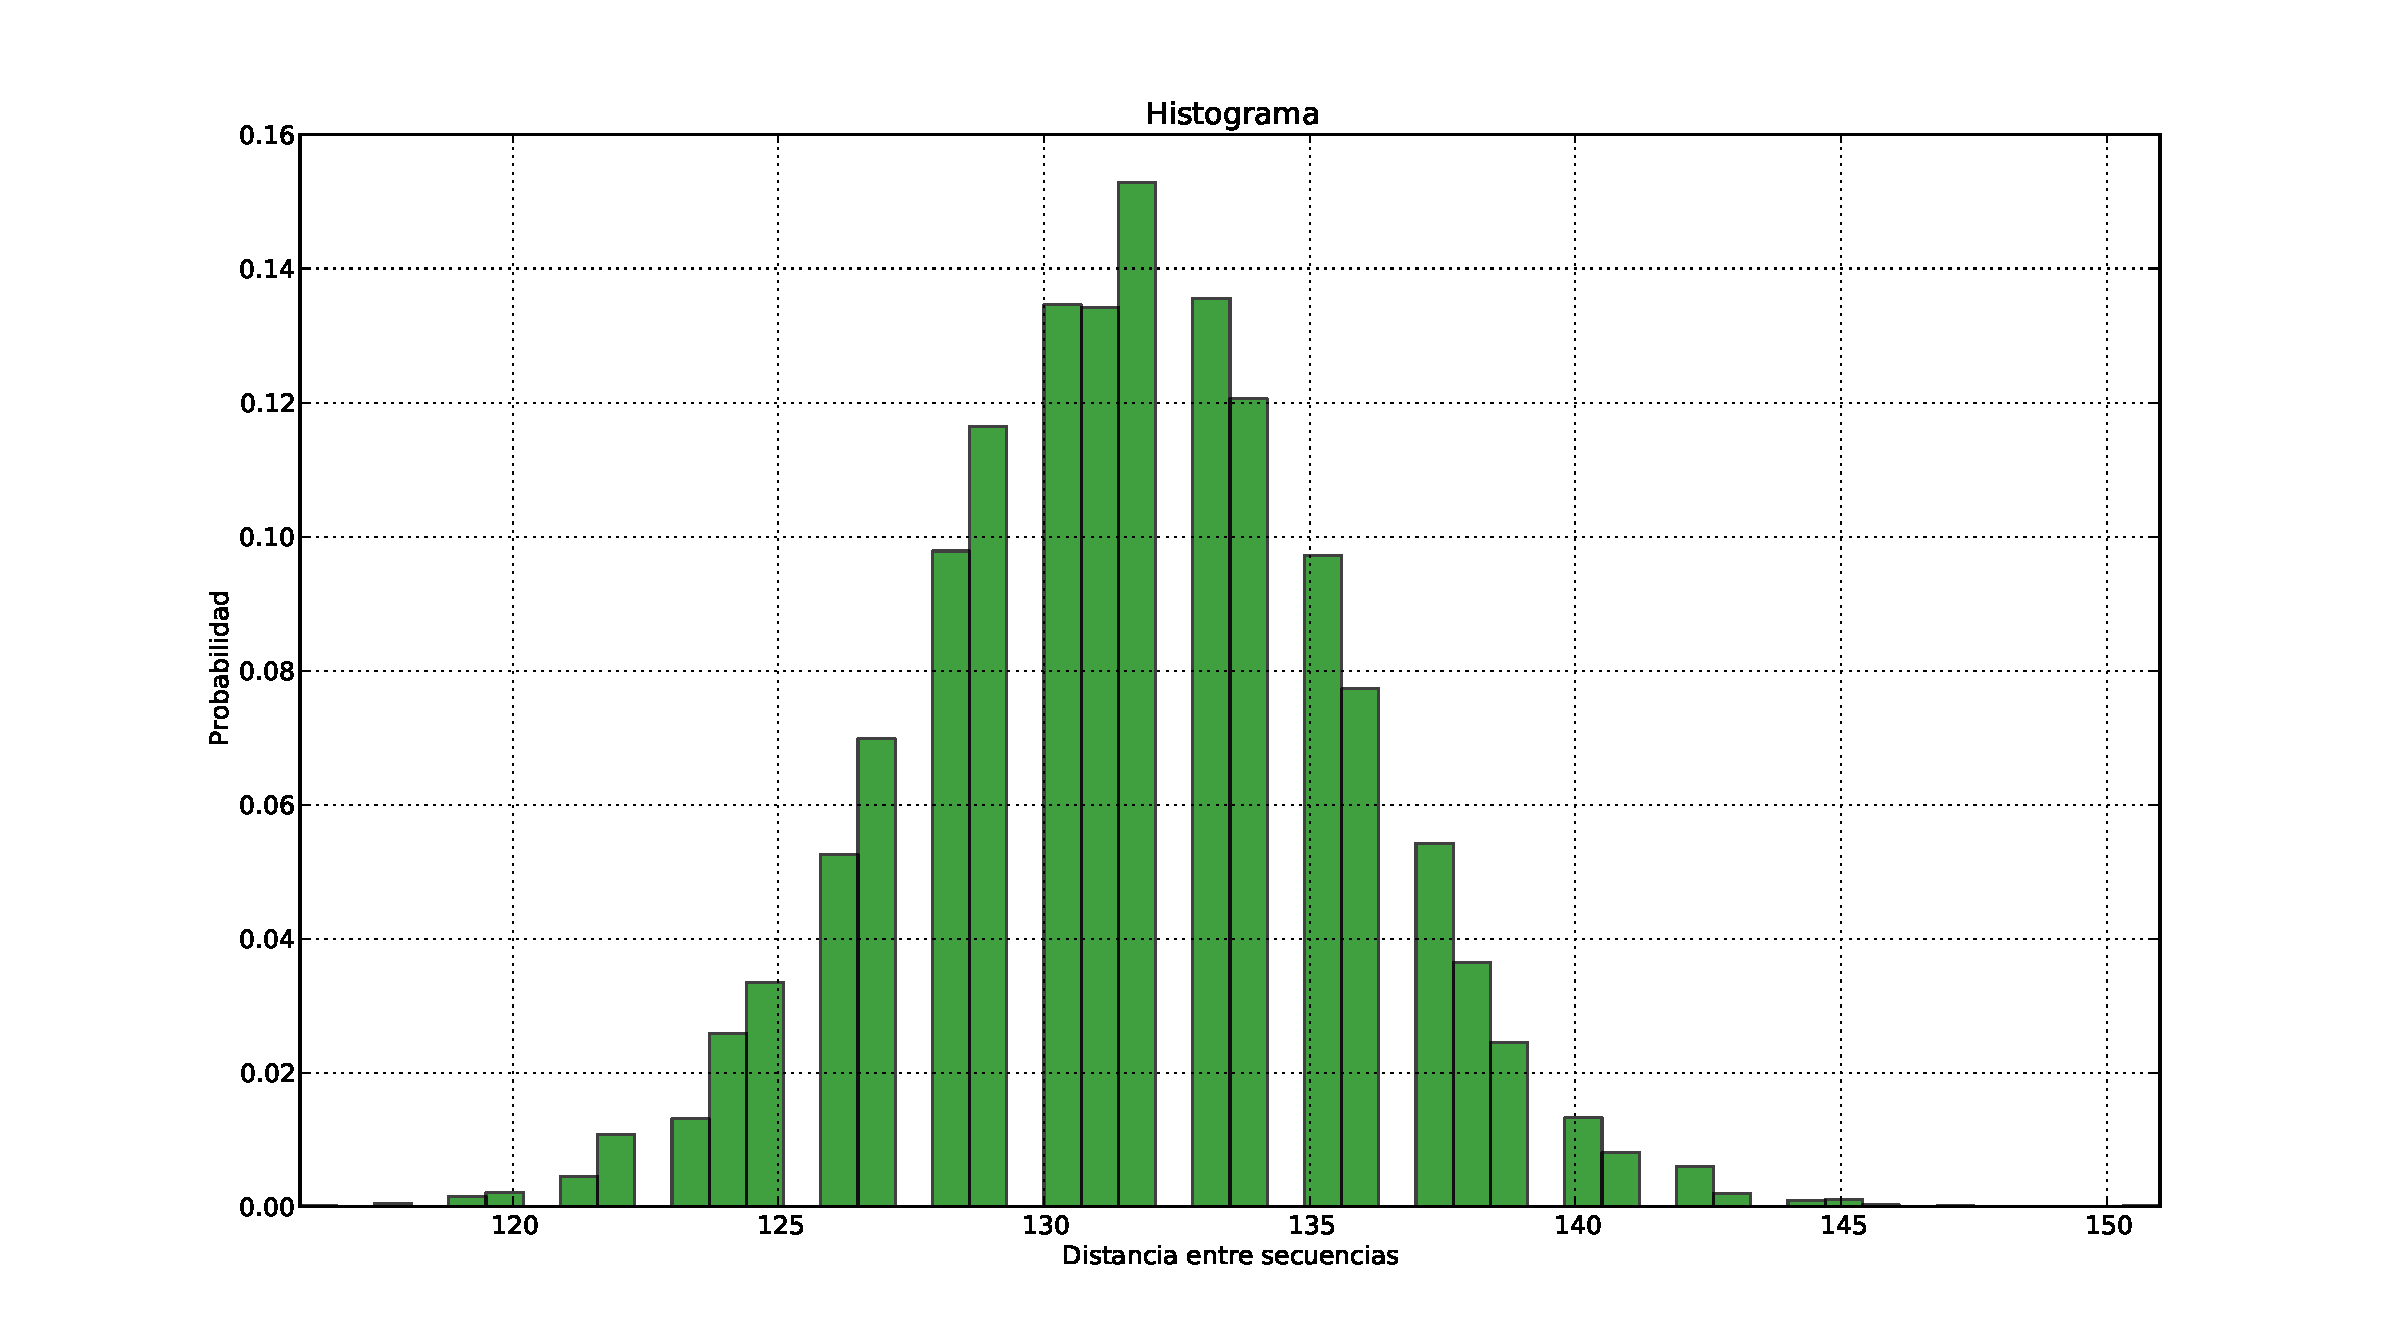
\includegraphics[width=\textwidth]{scripts/pregunta-2-3.pdf}
		\end{center}

		La información correspondiente del histograma y la aplicación es la siguiente:

		\begin{center}
		\begin{tabular}{|l|c|}
		\hline
		Largo 			 & 10000   \\\hline
		Media  			 & 131.547 \\\hline
		$\sigma$ 		 & 3.993   \\\hline
		Menor distancia  & 116.0   \\\hline
		Mayor distancia  & 151.0   \\\hline
		Tiempo ejecución & 4262.16 [sec] \\\hline
		\end{tabular}
		\end{center}

	\item Considerando (b) y (c), ¿por sobre qué valor de M diría usted que el parentesco entre las
		secuencias es indetectable?

		\blue{Respuesta:}

		\red{TO DO:} Completa


\end{enumerate}
